@@ -1,465 +0,0 @@
\appendix
\section{Tables}\label{Appendix:Tables}
\subsubsection{Gregor -- Keyboard Shorcuts}
{
\begin{table}[ht]
    \centering
    \resizebox{\textwidth}{!}{\begin{tabular}{| p{0.35\linewidth} | p{0.6\linewidth} |}
      \hline
      % after \\: \hline or \cline{col1-col2} \cline{col3-col4} ...
      Key & Action \\
      \hline
      \multicolumn{2}{|c|}{The File Menu} \\
      \hline
      Ctrl + O & Open an existing document \\
      Ctrl + S & Save the document to the last selected file or a new file if no previous file is associated. \\
      Ctrl + Shift + S & Save the data in a new file \\
      Ctrl + I & Import spline data from file \\
      Ctrl + E & Open up the export menu \\
      Shift + Del  & Clear the workspace \\
      Alt + F4 & Close the application \\
      \hline
      \multicolumn{2}{|c|}{The View Menu} \\
      \hline
      Ctrl + 4 & Combined Mode; Shows both ink and curves \\
      Ctrl + 5 & Ink Only Mode; Shows Only the ink marks and hides the curve alogwith the handles \\
      Ctrl + 6 & Splines Mode. Hides the ink marks \\
      Ctrl + G & Toggle the visibility of the grid \\
      Ctrl + Shift B & Toggle the visibility of the background images \\
      \hline
      \multicolumn{2}{|c|}{The Edit Menu} \\
      \hline
      Ctrl + 1 & Toggles the splines anchor centers \\
      Ctrl + 2 & Toggles the splines curvature handles \\
      Ctrl + 3 & Toggles the rotation handles \\
      Ctrl + V & Toggles the action of mouse left click between adding the anchor and dragging the workspace. \\
      \hline
      \multicolumn{2}{|c|}{Help}\\
      \hline
      F1 & Shows quick help \\
      F2 & Opens up the project Git.\\
      \hline
    \end{tabular}}
    \label{Table:Keyboardshortcuts}
    \end{table}
}
\clearpage
\section{Source Code}\label{Appendix:sourceCode}
{
    \clearpage
}
\section{Code Snippets}\label{Appendix:CodeSnippets}
{
\begin{lstlisting}[language=XML]
//Sample code of a rotating Bezier spline that will render the Urdu letter Aa'en in Nastaleeq.
<spline>
    <FlatTipWidth>150</FlatTipWidth>
    <Color>-5658199</Color>
    <anchor>
      <rotationoffset>0</rotationoffset>
      <P>-198.3791, 452.6993</P>
      <C1>-131.6351, 572.4461</C1>
      <C2>-265.1234, 332.9534</C2>
      <R1>-148.3791, 452.6993</R1>
    </anchor>
    <anchor>
      <rotationoffset>0</rotationoffset>
      <P>-296.5323, 156.2775</P>
      <C1>-439.8357, 254.4304</C1>
      <C2>-119.5302, 35.04326</C2>
      <R1>-246.5322, 156.2775</R1>
    </anchor>
    <anchor>
      <rotationoffset>0</rotationoffset>
      <P>25.40986, 374.1774</P>
      <C1>-47.22344, 262.2825</C1>
      <C2>98.04301, 486.0714</C2>
      <R1>75.40986, 374.1774</R1>
    </anchor>
    <anchor>
      <rotationoffset>0</rotationoffset>
      <P>-233.7143, -183.332</P>
      <C1>-208.1945, -28.25013</C1>
      <C2>-274.7982, -432.9961</C2>
      <R1>-183.7143, -183.332</R1>
    </anchor>
    <anchor>
      <rotationoffset>0</rotationoffset>
      <P>315.9428, -517.0526</P>
      <C1>95.77186, -679.5702</C1>
      <C2>435.6645, -428.6809</C2>
      <R1>365.9427, -517.0526</R1>
    </anchor>
    <anchor>
      <rotationoffset>0</rotationoffset>
      <P>441.5787, -144.0708</P>
      <C1>388.576, -277.5591</C1>
      <C2>494.5813, -10.58265</C2>
      <R1>491.5787, -144.0708</R1>
    </anchor>
  </spline>
\end{lstlisting}
}
\section{Images}
{

\begin{figure}[H]
  \centering
  \includegraphics[width=0.8\textwidth]{../Images/Nastaleeq_Ink.pdf}
  \caption
  {
      Nastaleeq sample by Gohar Qalam. (a) Original calligraphy photo. (b) Original photo processed for analysis. (c) Traced rotating bezier spline ink. (d) Difference between (b) and (c). The red pixel indicate the portions that are missing in (c) but are present in (b) and the blue ones show the missing pixels in (b) but are present in (c).
  }
\end{figure}

\begin{figure}[H]
  \centering
  
\includegraphics[width=0.8\textwidth]{../Images/Nastaleeq_Machined.pdf}
  \caption
  {
      Machined Nastaleeq sample by Gohar Qalam. (a) Rasterized rotating bezier spline for machining (b) Ink marks machined by a simulated robotic manipulator. (c) and (d) are differences between simulated ink mark and the rasterized photo and the processed original photo respectively. The red pixel indicate the portions that are missing in (c) but are present in the reference image and the blue ones show the missing pixels in reference but are present in the ink mark.
  }
\end{figure}

\begin{figure}[H]
  \centering
  
\includegraphics[width=0.8\textwidth]{../Images/Thuluth_Ink.pdf}
  \caption
  {
      Thuluth sample by Gohar Qalam. (a) Original calligraphy photo. (b) Original photo processed for analysis. (c) Traced rotating bezier spline ink. (d) Difference between (b) and (c). The red pixel indicate the portions that are missing in (c) but are present in (b) and the blue ones show the missing pixels in (b) but are present in (c).
  }
\end{figure}

\begin{figure}[H]
  \centering
  
\includegraphics[width=0.8\textwidth]{../Images/Thuluth_Machined.pdf}
  \caption
  {
      Machined Thuluth sample by Gohar Qalam. (a) Rasterized rotating bezier spline for machining (b) Ink marks machined by a simulated robotic manipulator. (c) and (d) are differences between simulated ink mark and the rasterized photo and the processed original photo respectively. The red pixel indicate the portions that are missing in (c) but are present in the reference image and the blue ones show the missing pixels in reference but are present in the ink mark.
  }
\end{figure}
}
\section{Gregor -- A short user manual}\label{Appendix:Gregor}
\subsection{Features}
{
    From a developer's perspective there are some features that are either implemented inevitably along the way of implemented the essential features or the usability of these features outweighs the additional effort required for the implementation. For example, the developer would have to program at least one color that the view-port will use to visualize the splines. The effort required to just expose the color option to the user is negligible as compared to writing the rendering engine. Many such features were also made a part of Gregor.

    \begin{itemize}
    \item Toggling the visibility of curvature and rotation handles.
    \item Toggling the visibility of ink-marks.
    \item Changing the opacity and color ink-marks.
    \item Changing the viewing mode between editing and viewing.
    \item Grid snapping with an option to be toggled on or off.
    \item Changing the rendering mode of rotating bezier splines.
    \item Selecting, moving, deleting, hiding and enabling individual splines.
    \item Document explorer with thumbnails of every spline in the document.
    \item Importing splines into existing workspace
    \item Selecting, moving, deleting, hiding and enabling individual splines.
    \item Application menu to change options with keyboard shortcuts to most used menu items
    \end{itemize}
}
\subsection{Usage}
{
    The software can be used to create/trace new splines and also open up existing ones. The software uses Microsoft XML format to store data. While creating or editing a spline, the user adds more anchors by clicking on the desired position on the document. Anchors can be added to previous splines as well as the one under focus. Once a spline has been created, the user can change the thickness and color of the ink-mark and then fine tune the position of each anchor point to match the desired stroke. To trace the strokes of an existing document, the user can also load images on to the background of the document and resized and positioned at the desired position.

    Once some splines have been created, the user can choose to save the work as XML documents or be exported as images. The user can also compare the newly created artwork with the background images to analyze the false positive and false negative areas. The analysis tools can preview the difference and compute the number of pixels in each difference image.
}
\subsection{Interface}
{
    The view of the software is the spline editor with a detailed main menu as shown in Fig. \ref{Fig:GregorInterface}, document summary and a list of most commonly used toggle buttons. The application also provides some keyboard shortcuts for the most frequently used toggle options like changing the visibility of different elements and toggling the editing modes.

    The information a rotating spline contains is too much to be viewed simultaneously. The center point of the anchors, the curvature handles, twist handles, the curve, the inkmark and the background image, when displayed simultaneously is just chaotic. On top of that, when all of these elements are interactive, using a single mouse cursor to interface becomes a headache. This is why the application presents viewing and editing modes.
    \subsubsection{The Viewing Modes}
    {
        The viewing modes can be controlled using options (g1) through (g3) as shown in Fig.  \ref{Fig:GregorInterface}, the ``View'' menu (a2), or the keyboard shortcuts. There are essentially three modes of view.
        \begin{itemize}
          \item (g1) is ink and curve mode. In this mode, the splines curves and the selected handles will be shown alongwith the ink marks.
          \item (g2) is ink-only mode. In this mode, the curvature handle of the splines alongwith the anchors and the handles are hidden.
          \item (g3) is curve-only mode. The inkmark will be hidden in this mode and only the curve alongwith the selected handles will be visible.
        \end{itemize}
        it is obvious that only one mode can be activated at a moment and it can be selected either from the options (g1) through (g3) in Fig.  \ref{Fig:GregorInterface} or through the View menu. Instead of clicking on the toggle buttons, using the keyboard shortcuts can sometimes be even more convenient.
    }
    \subsubsection{The Editing Modes}
    {
        The editing models enable or disable the anchors, curvature handles and the twist handles. As shown in Fig. \ref{Fig:GregorInterface} (h1) through (h3), the editing mode toggle buttons can be used to enable or disable any of these handles. Just like the editing modes, these modes can also be controlled using the keyboard shortcuts. Unlike the viewing modes, however, these modes can be enabled all at a time. It must be noted that while in ink-only mode, none of the editing modes will have any effect of the usability of the editing handles.
    }

    \begin{figure}
      \centering
      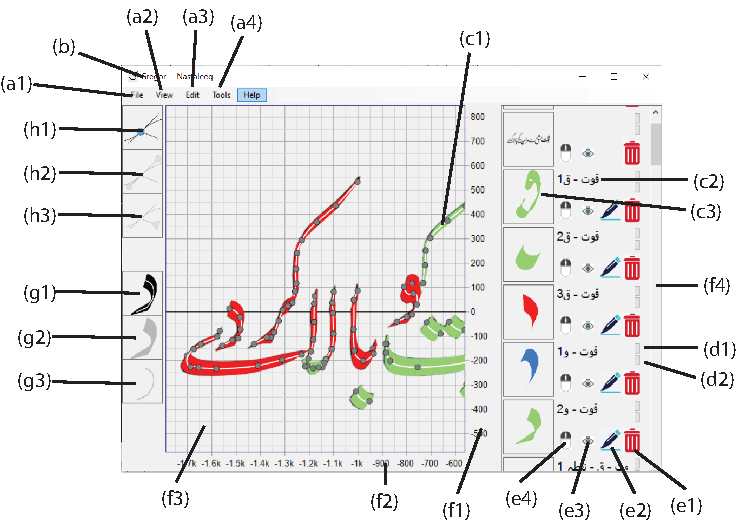
\includegraphics[width=0.9\textwidth]{../Images/GregorInterface.pdf}
      \caption{(a1-a4) The main menu options: (a1) Contains the options to open, save, import, export and clear splines and background images, (a2) enlists some viewing options; the ink viewing modes, visibility different elements of the workspace, visibility of background images, opacity of the ink-marks and rendering algorithm (a3) contains options related to editing on the workspace. It has the option to change the spline editing modes, the behaviour of left click on the workspace, and whether the splines can be dragged or not. (a4) has some analysis tools. (b) is the name of the currently open document. (c) is the main view of each spline in the document, (c2) and (c3) are the name of each spline element and its thumbnail respectively. (d1) and (d2) change the vertical order (z order) of the elements. While hovering the cursor over overlapping splines, the spline with higher position in the list will receive mouse event earlier. (e1), (e2), (e3) and (e4) are used to toggle editability, change visibility, modify color and thickness and delete the respective spline curve respectively. (f1) and (f2) are x and y axis of the workspace. (f3) is the main viewport. (f4) is the list of all the splines and images in the document. (g1) switches the view mode to both spline and inkmark, (g2) changes the viewing mode to ink only. (g3) changes the viewing mode to spline only. (h1), (h2) and (h3) toggle the visibility of center of anchor, curvature handle and the twist handle of the splines.
      } \label{Fig:GregorInterface}
    \end{figure}

}
\subsection{Modifying A Spline Curve}
{
    The application opens up an empty document by default. The first path one may choose to follow is to create new splines. This is done by adding new anchors. Anchors are added by simply clicking on an empty area of the screen. It must be noted that by default, the behaviour of the left mouse click must be switched from the Edit menu or using the keyboard shortcut to enable ``Add anchors using left mouse click''. Once an anchor has been added, adding a second anchor automatically creates a spline between the previously added anchor.
    \subsubsection{Starting a New Curve}
    {
        Since each click will append an anchor at the end of to the current spline, to break the curve and start a new one, some other procedure must be adopted. This can either be done by right clicking on an empty part of the document or toggling the ``Add anchors using left mouse click'' option off and quickly using the keyboard shortcut.
    }
    \subsubsection{Appending to a Previously Active Curve}
    {
        To append anchors at the end or the beginning of a previously active spline, simple click the center point of the first or the last center of anchor of the desired curve and it will be selected. Now, every new click will append to the selected curve just like before.
    }
    \subsubsection{Adding Anchors in the Middle}
    {
        Unfortunately adding anchor amid a curve is not a possibility yet. It would require an algorithm that can compute the nearest point on a curve from the mouse position that can show where the new anchor will be added. A work-around for now is to add anchors at the beginning or the end and soft the existing anchors inward until one of them reaches the required position.
    }
    \subsubsection{Simultaneous Curve Editing While Adding New Anchors}
    {
        It is usually very convenient to add an anchor while dragging the mouse cursor at the same time. This way, the software first adds an anchor just like it should on a mouse click but by dragging the cursor, instead of dragging the center of the newly added anchor, it drags the respective curvature handle instead. Creating new long strokes is very convenient this way. Please note that for this trick, the viewing mode must be showing the curve and both the centers and curvatures handles should be enabled.
    }
}
\subsection{Modifying an Ink-mark}
{
    \subsubsection{Adding an Ink-Mark}
    {
        Once a spline has been created with two or more anchors, the viewing mode can be switched to show ink and curve and the twist handle can be enabled while disabling the curvature handle. This will not convert the spline to a rotating curve unless it has been given a thickness. To change the thickness of a spline, simply click on it or the respective appearance in the document explorer as shown in Fig. \ref{Fig:AppearanceEditor} (e3). A curve appearance editor will pop up as shown in Fig. . Allowing to change both the broad edge thickness and the color of the ink-mark.

        \begin{figure}
          \centering
          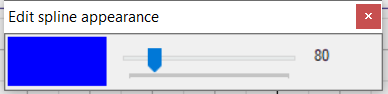
\includegraphics[width=0.3\textwidth]{../Images/appearance editor.PNG}
          \caption{The curve appearance editor lets the user modify the color and broad edge thickness of the simulated pen} \label{Fig:AppearanceEditor}
        \end{figure}
    }
    \subsubsection{Modifying the twist/rotation}
    {
        Once the Ink-mark has some thickness, it will start to show up on the viewport as well. If the rotation handles are enabled, one can start dragging each rotation handle to start twisting the curve. The artist usually continuously switches between ink and curvature handles to keep modifying the final spline until they are satisfied with the final ink-marks.
    }
}
\subsection{Using Images}
{
    Images can be imported to an existing workspace by simply selecting the menu option File > Import > Image. One can choose to import an image directly from an image file or the clipboard if the user has already copied an image using a graphics editor like a photoshop or Microsoft Paint. To view it, the background images must also be enabled from the Edit menu. Once the image is visible, the user can select a discrete handle at the middle of the image to change the placement and an anchor at the top right corner to change the size, aspect ratio, mirroring and rotation of the image.
}
\subsection{Using the Document Explorer}
{
    In addition to shoing up in the viewport, all the images and splines also appear in the document explorer as shown in Fig. \ref{Fig:GregorInterface} (f4). Each item is represented by a multi-option control which shows some controls associated with the respective item.
    \begin{itemize}
      \item Fig. \ref{Fig:GregorInterface}(c3) is a normalized thumbnail of the respective item.
      \item One can change the name of each item using Fig. \ref{Fig:GregorInterface}(c2) which can come handy while dealing with multiple items which may look similar.
      \item (e1) will delete the respective item
      \item (e2) pops up the appearance menu of the respective curve
      \item (e3) toggles the visibility of the respective item
      \item (e4) toggles the editability of an item. A Disabled item can be viewed but not interacted with.
      \item (d1) and (d2) change the order of the z-order items in a document. A simple trick while moving an item in a very long list of items is to click once on the required move button and then instead of finding the relocated button again and clicking on it again, one can now choose to press the space bar or the enter button on the keyboard which will press the button again no matter where-ever it is.
    \end{itemize}

}
\subsection{Save, Load, Export}
{
    Once the user is satisfied with the artwork, they can save it using the File menu. Once saved, the user can save any further changes to the same file by simply using the well known save command ``Control + S'' or by using the Save option from the menu again. Once saved, the file can either be opened by using the Open option in the File menu or using the windows explorer. The saved files use an extension ``rbs''. The windows usually does not recognize this extension and will thus present a list of typical applications that can open it. Choose to browse for a custom application and point to the Gregor executable. The windows will not only open the file in Gregor but also remember this choice to open rbs files in the future.

    In addition to opening a file, a user can choose to import the curves contained in a file into an existing workspace, No current items will be cleared while importing a file.

    \subsubsection{Exporting Images}
    {
        Since the curves are vector data, one may still need to export this vector into a rasterized image to be used in various circumstances. A user can export the workspace in a pixel depth of their choice using the export option in the File menu. The export window as shown in Fig. \ref{Fig:ExportMenu} presents several options
        \begin{itemize}
          \item User can control whether to include the anchors and spline curves in the render
          \item The background images can also be exported alongwith the splines.
          \item A uniform color can be selected for the exported splines.
          \item The user can also specify the rendering algorithm for the ink-mark.
          \item Last but not the least, the user can specify a pixel density. By default, each unit on the grid will be considered one pixel. Specifying a pixel density of $100$~DPU specifies to generate one hundred pixels between one unit on the grid. It must be noted that while using too dense or too large images, the application might succumb to the memory load of the procedure. So it is wise to always save the data before attempting to export an image.
        \end{itemize}

        \begin{figure}
          \centering
          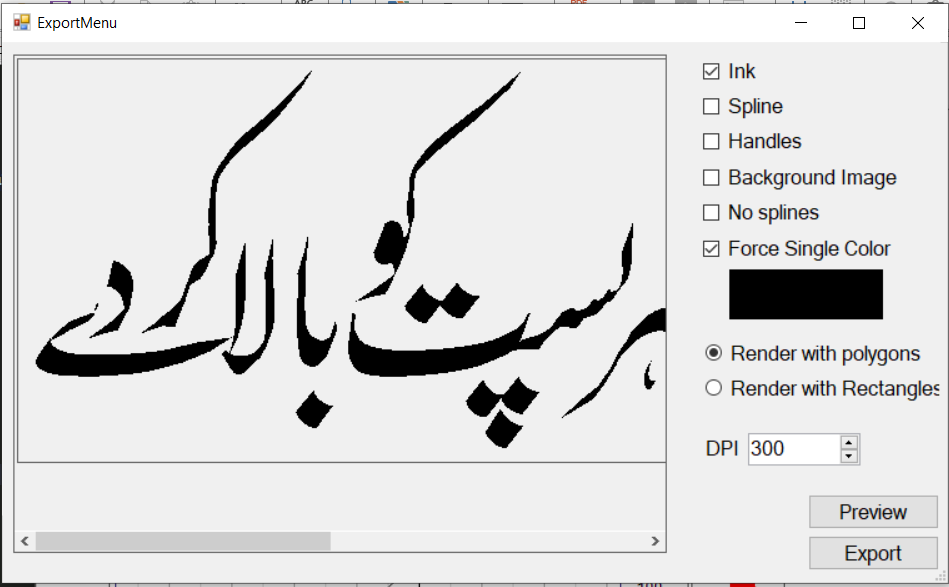
\includegraphics[width=0.9\textwidth]{../Images/ExportMenu.PNG}
          \caption{The curve appearance editor lets the user modify the color and broad edge thickness of the simulated pen} \label{Fig:ExportMenu}
        \end{figure}
    }
    \subsubsection{The File Format}
    {
        Gregor uses Microsoft XML format to save data. XML is primarily used to save text data. To pack images in it, the image is first converted into a hexadecimal list of byte data and represented as a very long string. It may inconvenience the user if they try to open it using a simple text editor which will show thousands of lines of gibberish hexadecimal bytes. One way to open the file as text is to open using an advanced raw text editor like Notepad++ or Sublime Text. These editors have the provision to collapse a certain node of an XML document, making the rest of the data more readable.
    }
}
\clearpage 